\documentclass[fontsize=11]{article}
\usepackage{amsmath,amssymb, mathtools}
\usepackage{tabularx}
\usepackage{hyperref}
\begin{document}

\section{Rules of thumb}

\begin{tabularx}{\linewidth}{X c c}
Rule of Thumb & source & notes \\
If you have more than 1M datapoints - use deep learning
dealing with images / audio / video), then you’re probably better off learning deep learning. & \href{https://www.quora.com/Should-a-machine-learning-beginner-go-straight-for-deep-learning}{link} & \\
``I've seen over and over that
 one of the most reliable ways to
 get a high performance machine learning
 system is to take
 a low bias learning algorithm
 and to train it on a massive training set.'' & Andrew Ng & \\
 ``if you don't have a low bias algorithm, try to add more features'' & Andrew Ng & \\
 "the process of artificial
 data synthesis it is .. a little bit of
 an art as well and sometimes
 you just have to try it and see if it works." & Andrew Ng & \\
  "try to calculate how much time it would take to collect and label data yourself" & Andrew Ng & \\
 ``It's not who has the best algorithm that wins. It's who has the most data '' & & \\
 
\end{tabularx}

\section{Resources}

\begin{tabularx}{\linewidth}{X|c|c}
Topic & link & notes \\
Data science project ideas & \href{https://www.quora.com/What-are-some-really-interesting-machine-learning-projects-for-beginners}{link} & \\
\end{tabularx}

\section{Week 6 - Machine Learning Diagnostics}

\subsection{Learning Curves - figuring out if you have high bias or high variance}
Plot error versus m (training set size). 

High bias looks like this:
\begin{figure}
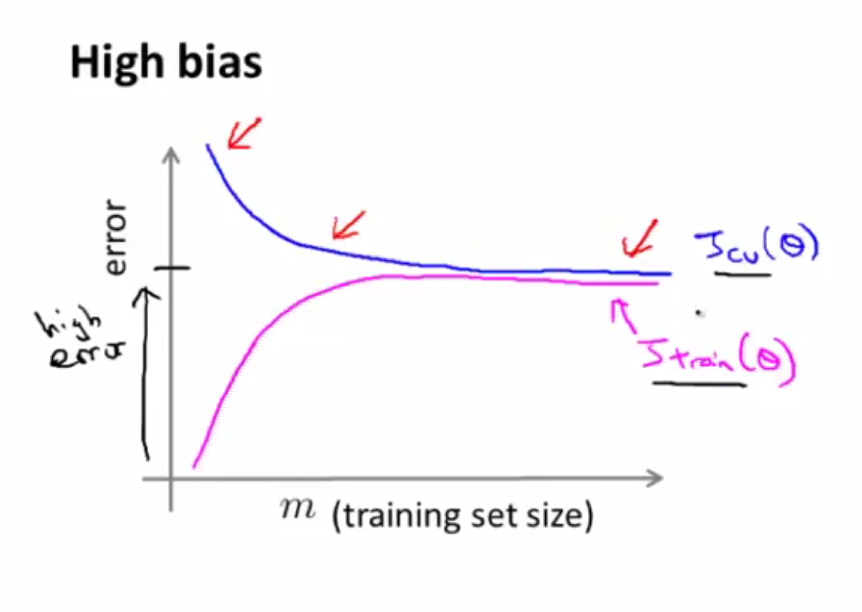
\includegraphics[scale=1]{./figures/high_bias.png}
\end{figure}

Getting more data won't help.

High variance looks like this:
\begin{figure}
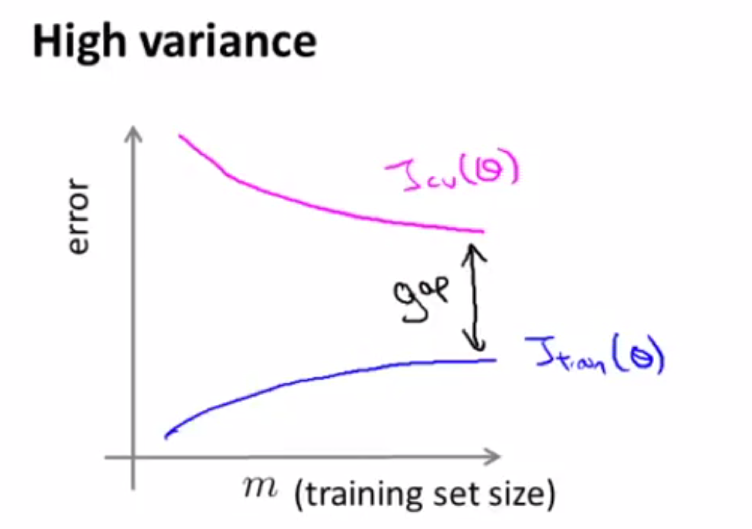
\includegraphics[scale=1]{./figures/high_variance.png}
\end{figure}

Getting more data is likely to help.

 To plot a learning curve, $J_{\mathrm{train}}(\theta)$ average squared error on my training
 set or Jcv which is
 the average squared error on my cross validation set.
 And I'm going to plot
 that as a function
 of m, that is as a function
 of the number of training examples I have.
 And so m is usually a constant like maybe I just have, you know, a 100
 training examples but what I'm
 going to do is artificially with
 use my training set exercise. So, I
 deliberately limit myself to using only,
 say, 10 or 20 or
 30 or 40 training examples and
 plot what the training error is and
 what the cross validation is for this
 smallest training set exercises. 
 
\subsection{Debugging a learning algorithm}

\begin{itemize}
\item Get more training examples - fixes high variance
\item try smaller sets of features - fixes high variance
\item Try getting additional features - fixes high bias
\item Try adding polynomial features - fixes high bias
\item try decreasing $\lambda$ - fixes high bias
\item try increasing $\lambda$ - fixes high variance
\end{itemize}

Neural networks:
Often the larger the better (i.e. more hidden units the better), and use regularization to address overfitting.

How to choose how many hidden layers:
\begin{itemize}
\item[] use one, hidden layer (often this is enough) measure error, 
\item[] use 2 measure error etc.
\item[] $\vdots$
\end{itemize}

\subsection{Skewed Classes}
We have a lot more examples from one class compared to another.

If you have skewed classes, don't simply use classification accuracy as an evaluation metric. Instead use Precision/Recall. 

\paragraph{Precision}
of all the patients where we predicted y=1, what fraction actually has cancer?

\begin{align*}
\frac{\mathrm{True \ Positives}}{\# \mathrm{\ predicted \ postive}} = \frac{\mathrm{True \ Positives}}{\mathrm{True \ Positives} + \mathrm{False \ pos}}
\end{align*}

\paragraph{Recall}
Of all patients that actually have cancer, what fraction did we correctly detect as having cancer?

\begin{align*}
\frac{\mathrm{True \ Positives}}{\# \mathrm{actual \ postives}} = \frac{\mathrm{True \ Positives}}{\mathrm{True \ Positives} + \mathrm{False \ Neg}}
\end{align*}

y=1 denotes presence of rare class, e.g. patient has cancer.

High precision and high recall = good classifier

\paragraph{F score }
How to use precision and recall to come up with a single real number evaluation metric

Could use average, but not really a good idea, you'll get a number which is biased towards extreme values (e.g recall = 1, precision = 0.02).

\begin{align*}
F_1 = 2 \frac{PR}{P+R}
\end{align*}
Both P \& R have to be high for $F_1$ to be high
There are a lot of ways to combine precision and recall, but this is a very common one.

\subsection{very large datasets}
Assumption: If features have enough information to accurately predict $y$

If a human expert had the information contained in the features, would they have enough information to predict y? If yes, then the above assumption is true. 

Then use a low bias algorithm, like a neural network with lots of hidden nodes or linear regression with lots of features. 

If assumption 1 holds and you have a low bias algorithm, then getting lots of data is likely to really help your dataset.

\section{Week 7: Unsupervised Learning }

Example Applications of Clustering
\begin{itemize}
\item Market Segmentation
\item Social network analysis
\item Organize Computing clusters
\item Astronomical data analysis
\end{itemize}



\section{Week 9:Anomaly Detection }
Anomaly Detection Example:
$p(x_{test}) < \epsilon $ flag anomaly
$p(x_{test}) \geq \epsilon $ flag anomaly

Most frequent use: 
\begin{itemize}
\item Fraud Detection:
$x^{(i)}$ = features of user $i$'s activities
Model $p(x)$ from data
Identify usual users by checking which have $p(x) < \epsilon$

\item Manufacturing 

\item Monitoring computers in a data center
$x^{(i)}$ features of machine $i$
$x_1$ memory use,$ x_2$ number of disk accesses .
\end{itemize}

\subsection{Normal distribution}

\subsection{Parameter Estimation}
For Normal Distribution

(These are Maximum likelihood estimates - they are just averages)

\begin{align*}
\mu &= \frac{1}{m} \sum_{i=1}^m x^{(i)}
\end{align*}

\begin{align*}
\sigma^2 = \frac{1}{m} \sum_{i=1}^m  (x^{(i)} - \mu)^2
\end{align*}

\subsection{Density estimation}
training set: $\{x^{(i)},\dots, x^{(m)} \}$
each example is $x \in R^n$

\begin{align*}
p(x) &= p(x_1; \mu_1,\sigma_1^2)p(x_2, \mu_2,\sigma_2^2)\dots p(x_n, \mu_n,\sigma_n^2)\\
&= \prod_{j=1}^n p(x_j ; \mu_j, \sigma_j^2)
\end{align*}

The above corresponds to assumption that: 
\begin{align*}
x_1  &\backsim \mathcal{N}(\mu_1, \sigma_1^2) \\
x_2  &\backsim \mathcal{N}(\mu_2, \sigma_2^2) \\
      &\vdots
\end{align*}
which corresponds to an independence assumption on the input features.

\subsubsection{Anomaly detection algorithm}
\begin{enumerate}
\item Choose features $x_i$ which you think might be indicative of anomalous examples, where each $x_i \in R^n$
\item Fit parameters $\mu_1, \dots, \mu_n, \sigma^2_1, \dots, \sigma^2_n,$, i.e. compute:
\begin{itemize}
\item[] $$ \mu_j = \frac{1}{m}\sum_{i=1}^m x_j^{(i)}$$
where $\mu_j$ is the average value of the $j$th feature.
\item[] $$ \sigma_j^2 = \frac{1}{m}\sum_{i=1}^m (x_j^{(i)} - \mu_j)^2 $$
\end{itemize}
\item Given new example $x$, compute $p(x)$:
$$ p(x) =  \prod_{j=1}^n p(x_j ; \mu_j, \sigma_j^2) = \prod_{j=1}^n \frac{1}{\sqrt{2\pi}\sigma_j} \exp \left(-\frac{(x_j - \mu_j)^2}{2\sigma^2_j} \right)$$ 
anomaly if $p(x) < \epsilon$
\end{enumerate}

\section{Notes Coursera Week 10: Large Scale Machine Learning }

\subsection{Vid1: Learning with Large Datasets}
motivating example:
m = 100,000,000

\begin{align*}
\theta_j := \theta_j - \alpha \frac{1}{m} \sum_{i=1}^m (h_{\theta}(x^{(i)} - y^{(i)}))x_j^{(i)}
\end{align*}

That's 100,000,000 summations for 1 step of gradient descent.

Idea: train on 1000 samples, maybe it will do just as well. 

Quiz question: Suppose you have m=100,000, 000; how can you tell if using all of the data is likely to perform much better than using a small subset of the data (m= 1000).

Answer: Plot a learning curve for a range of values of m and verify that the algorithm has high variance when m is small. 

\begin{figure}
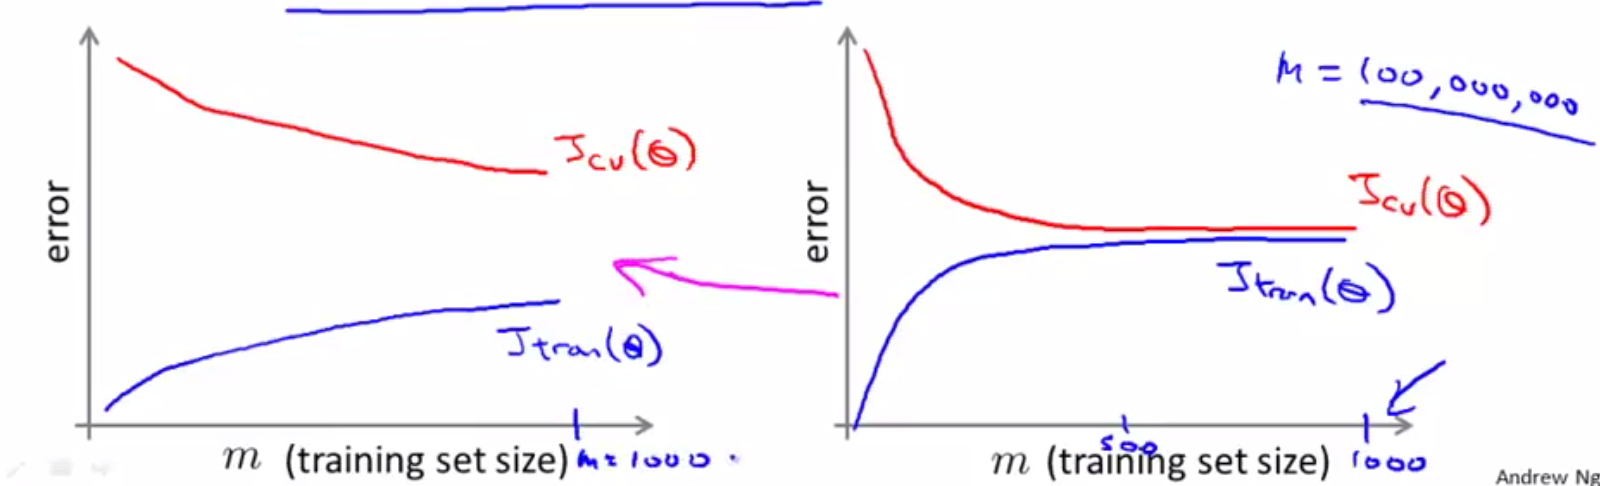
\includegraphics[scale=0.3]{./figures/learning_curves.png}
\caption{Left: High variance, should add more data, Right: high bias, more data won't help, should add more features, or more hidden units to neural networks}
\end{figure}


\subsection{Vid2: Computationally efficient methods: Stochastic Gradient Descent}
Gradient descent not efficient for very large datasets.
It's called `Batch gradient descent'


\begin{tabularx}{\linewidth}{l|X|}
$ J_{train}(\theta) $ & stuff 
\end{tabularx}

 


\subsection{Vid3: Mini-Batch Gradient Descent}

\subsection{Vid4: Stochastic Gradient Descent Convergence}

\subsection{Vid5: Online Learning}

\subsection{Vid6: Map reduce and Data Parallelism}

\section{Week 11: Where to allocate scarce resources?}
Video title: Ceiling analysis: what part of the pipeline to work on next

Suppose you have pipeline of tasks in your machine learning project. And your current overall accuracy is 72\%. To figure out where to allocate resources to improve the system, break the pipeline and feed in perfectly correct information (by manually correcting the label outputs of the previous component for example) to one component, and recalculate the performance improvement of the entire pipeline. Then do the same with the next component, etc. etc. This will show you the 'upside potential' for each component. Allocate the resources to the component with the biggest upside potential.



\end{document}
